%
% Module 3 Chapter 5 Program Documentation
% CSC160-C00: Computer Science I (C++) (Jeffrey Hemmes)
% Author: Ashton Hellwig
% Date: 13 March 2020
%


\documentclass[a4paper, 11pt]{article}
  % Packages
  \usepackage[utf8]{inputenc}         % Encoding
  \usepackage[english]{babel}         % Internationalization
  \usepackage{times}                  % Times New Roman font
  \usepackage{soul}                   % Highlighting
  \usepackage{hyperref}               % Links (internal and external)
  \usepackage{fancyhdr}               % Headers and footers
  \usepackage[dvipsnames]{xcolor}     % Text Colors
  \usepackage{listings}               % Code Snippets
  \usepackage[section]{algorithm}     % For TOC support
  \usepackage{algpseudocode}          % Algorithmic notation environments
  \usepackage{enumitem}               % Ordered lists
  \usepackage{geometry}               % Page layout
  \usepackage{graphicx}               % Image support
  \usepackage{wrapfig}                % Sideways figures (landscape)
  \usepackage{lscape}                 % Sideways figures (landscape)
  \usepackage{rotating}               % Sideways figures (landscape)
  \usepackage{epstopdf}               % Sideways figures (landscape)
  \usepackage[toc, page]{appendix}    % Appendix
  \usepackage{setspace}               % Paragraph and line spacing
  \usepackage{bookmark}               % Required for appendix
  \usepackage{adjustbox}              % Required for appendix
  \usepackage{csquotes}               % Required for appendix
  \usepackage{amsthm}                 % Theorem environments
  \usepackage{array}                  % Arrays
  \usepackage{makecell}               % Table helpers
  \usepackage{amsmath}                % Mathematical symbols
  \usepackage[fleqn]{mathtools}       % Mathematical environments
  \usepackage{amssymb}                % Misc. symbols for logic and math
  \usepackage{relsize}                % Relative Sizing
  \usepackage{multicol}               % Multi-figure displays (grid)
  \usepackage{etoolbox,refcount}      % Required for mdframed
  \usepackage{parcolumns}             % Paragraph grids
  \usepackage{mdframed}               % Colored box environments
  \usepackage{float}                  % Floating Environments 
  \usepackage{aliascnt}               %
  % \usepackage[                        % Bibliography management
    % backend=biber,%
    % style=apa%
  % ]{biblatex}

  % Bibliography Setup
  % \addbibresource{main.bib}
  % \newcommand{\CiteSection}[2]{%
    % (\autocite{#1}, ~\S {#1})%
  % }

%   \UseRawInputEncoding

  % Tables
  \renewcommand\theadalign{bc}
  \renewcommand\theadfont{\bfseries}
  \renewcommand\theadgape{\Gape[4pt]}
  \renewcommand\cellgape{\Gape[4pt]}

  % Lists
  \newcounter{countitems}
  \newcounter{nextitemizecount}
  \newcommand{\setupcountitems}{%
    \stepcounter{nextitemizecount}%
    \setcounter{countitems}{0}%
    \preto\item{\stepcounter{countitems}}%
  }
  \makeatletter
  \newcommand{\computecountitems}{%
    \edef\@currentlabel{\number\c@countitems}%
    \label{countitems@\number\numexpr\value{nextitemizecount}-1\relax}%
  }
  \newcommand{\nextitemizecount}{%
    \getrefnumber{countitems@\number\c@nextitemizecount}%
  }
  \newcommand{\previtemizecount}{%
    \getrefnumber{countitems@\number\numexpr\value{nextitemizecount}-1\relax}%
  }
  \makeatother
  \newenvironment{AutoMultiColItemize}{%
  \ifnumcomp{\nextitemizecount}{>}{3}{\begin{multicols}{2}}{}%
  \setupcountitems\begin{itemize}}%
  {\end{itemize}%
  \unskip\computecountitems\ifnumcomp{\previtemizecount}{>}{3}{\end{multicols}}{}}



  % Colors
  \newcommand{\commentstylecolor}{\color{Gray}}
  \newcommand{\keywordstylecolor}{\color{MidnightBlue}}
  \newcommand{\stringstylecolor}{\color{ForestGreen}}
  \newcommand{\questioninput}{\color{Red}}
  \newcommand{\answertcolor}{\color{Green}}
  \newcommand{\myanswer}{\answertcolor{\hl}}

  % Symbols
  \newcommand{\answerflow}{\rotatebox[origin=c]{180}{$\Lsh$}}
  \newcommand{\toanswer}{\mathlarger{\mathlarger{\answerflow}}\quad}

  % Math
  \newcommand{\highlight}[1]{%
    \colorbox{green!50}{$\displaystyle#1$}}

  % Image Directory
  \graphicspath{ {screenshots/} }


  % Hyperlink Setup
  \hypersetup{
    colorlinks = true,
    urlcolor = blue,
    linkcolor = blue
  }


  % Algorithm Settings
  \newcommand{\pluseq}{\mathrel{{+}{=}}}
  \newcommand{\minuseq}{\mathrel{{-}{=}}}


  % Syntax-Highlighting for Code Snippets
  \lstset{
    backgroundcolor=\color{white},
    breaklines=true,%
    captionpos=b,%
    frame=tlrb,%
    tabsize=2,%
    numbers=left,%
    showstringspaces=false,%
    commentstyle=\commentstylecolor,%
    keywordstyle=\keywordstylecolor,%
    stringstyle=\stringstylecolor%
  }
  \lstset{literate=
  {á}{{\'a}}1 {é}{{\'e}}1 {í}{{\'i}}1 {ó}{{\'o}}1 {ú}{{\'u}}1
  {Á}{{\'A}}1 {É}{{\'E}}1 {Í}{{\'I}}1 {Ó}{{\'O}}1 {Ú}{{\'U}}1
  {à}{{\`a}}1 {è}{{\`e}}1 {ì}{{\`i}}1 {ò}{{\`o}}1 {ù}{{\`u}}1
  {À}{{\`A}}1 {È}{{\'E}}1 {Ì}{{\`I}}1 {Ò}{{\`O}}1 {Ù}{{\`U}}1
  {ä}{{\"a}}1 {ë}{{\"e}}1 {ï}{{\"i}}1 {ö}{{\"o}}1 {ü}{{\"u}}1
  {Ä}{{\"A}}1 {Ë}{{\"E}}1 {Ï}{{\"I}}1 {Ö}{{\"O}}1 {Ü}{{\"U}}1
  {â}{{\^a}}1 {ê}{{\^e}}1 {î}{{\^i}}1 {ô}{{\^o}}1 {û}{{\^u}}1
  {Â}{{\^A}}1 {Ê}{{\^E}}1 {Î}{{\^I}}1 {Ô}{{\^O}}1 {Û}{{\^U}}1
  {œ}{{\oe}}1 {Œ}{{\OE}}1 {æ}{{\ae}}1 {Æ}{{\AE}}1 {ß}{{\ss}}1
  {ű}{{\H{u}}}1 {Ű}{{\H{U}}}1 {ő}{{\H{o}}}1 {Ő}{{\H{O}}}1
  {ç}{{\c c}}1 {Ç}{{\c C}}1 {ø}{{\o}}1 {å}{{\r a}}1 {Å}{{\r A}}1
  {€}{{\euro}}1 {£}{{\pounds}}1 {«}{{\guillemotleft}}1
  {»}{{\guillemotright}}1 {ñ}{{\~n}}1 {Ñ}{{\~N}}1 {¿}{{?`}}1
}
  \newenvironment{alltt}{\ttfamily}{\par}
  \lstMakeShortInline[language=c++,columns=fixed]|

  % Page Configuration
  %% Style
  \pagestyle{fancy}

  %% Layout
  \geometry{%
    a4paper,%
    top=2.5cm,%
    bottom=2.5cm,%
    left=2.5cm,%
    right=2.5cm%
  }
  %%% Document
  \setlength{\headheight}{15pt}
  \setlength{\floatsep}{12pt}
  \setlength{\parindent}{2em}
  \setlength{\parskip}{0.5em}
  \renewcommand{\baselinestretch}{.9}

  %% Title page
  \title{Chapter 5 Programming Assignment Documentation}
  \author{Ashton Hellwig}
  \date\today
  \setcounter{tocdepth}{3}

  %% Subsequent pages
  \lhead{CSC160}
  \rhead{Computer Science I (C++)}
  \lfoot{M3C5Program}
  \rfoot{A. Hellwig}


  % Document Content
\begin{document}
  % Title Page
  \maketitle
  \tableofcontents
  \listofalgorithms
  \lstlistoflistings
  \listoffigures
  \newpage


  % Problem Analysis
  \section{Problem Analysis}
    The problem states:
    \begin{mdframed}[backgroundcolor=green!20]
      This assignment relates to content from Chapter 5 of the eText.

      \textbf{Instructions}\vspace{-8pt}
      \begin{enumerate}
        \item Review the general programming assignment instructions.
        \item%
          Write a program that uses |while| loops to perform the following
            steps:
            \begin{enumerate}[label=\alph*.]
              \item Prompt the user to input two integers: firstNum and
                secondNum (firstNum must be less than secondNum).
              \item Output all odd numbers between firstNum and secondNum.
              \item Output the sum of all even numbers between firstNum and
                secondNum.
              \item Output the numbers and their squares between 1 and 10.
              \item Output the sum of the square of the odd numbers between
                firstNum and secondNum.
              \item Output all uppercase letters.
            \end{enumerate}
      \end{enumerate}
    \end{mdframed}

    \subsection{Data}
      Placeholder.

    \subsection{Desired Output}
      \begin{lstlisting}[%
        language=bash,%
        columns=flexible,%
        caption={ashellwig\_m3c5\_programming\_assignment output %
          (stdout)},%
        label={desiredoutput:stdout}%
    ]
Enter two numbers.
First number must be less than the second number you enter
Enter numbers: <NUMBER1> <NUMBER2>

Odd integers between <NUMBER1> and <NUMBER2> are:
<ODD_INTEGERS>
Sum of even integers between <NUMBER1> and <NUMBER2> = <SUMEVENS>
Number     Square of Number
1                 1
2                 4
3                 9
4                16
5                25
6                36
7                49
8                64
9                81
10              100

Sum of the squares of odd integers between <NUMBER1> and <NUMBER2> = <SUMODDINT>
Upper case letters are: A B C D E F G H I J K L M N O P Q R S T U V W X Y Z

Press any key to continue...
      \end{lstlisting}


  % Algorithm
  \newpage
  \section{Algorithm}
    Below is the algorithm for the program.
    \begin{algorithm}[h]
      \caption{Chapter 5 Program Algorithm}
      \vspace{12pt}
      \begin{algorithmic}[1]
        % MAIN
        \Function{main}{}
          %% Variables
          \State $num1\gets0$\Comment{Variable Declarations}
          \State\Return{$num1$}
        \EndFunction
      \end{algorithmic}
      \label{alg:c3program}
    \end{algorithm}


  % User Documentation
  \newpage
  
  \section{User Documentation}
    Please see Appendix \ref{appendix:img} for images showing the compilation
      (Figure \ref{img:compilation}) and the running program (Figure
      \ref{img:running} and Figure \ref{img:running2}).

    %% Usage
    \subsection{Build}
      The following are instructions with two use cases:
      \begin{itemize}
        \item With GNU Make
        \item Bundled Release
      \end{itemize}
      \subsubsection{With GNU Make}
        \begin{enumerate}
          \item Navigate to the unzipped folder containing the project,
            \textbf{with a terminal emulator or command prompt}, this will
            (most likely) mean running:
            \begin{lstlisting}[language=bash]
cd ~/Downloads/ashellwig_m3c5_programming_assignment
            \end{lstlisting}
          \item Compile the program and documentation\footnote{\textbf{Note%
            }: This requires the whole \texttt{texlive} suite as well as
            \texttt{latexmk} to be installed.} using GNU automake after
            switching to the source directory:
            \begin{lstlisting}[%
              language=bash,%
              caption={Chapter 5 Program Build Commands},%
            ]
make debug

./out/bin/ashellwig_m3c5_programming_assignment.bin # Run program

make clean-all # Removes object files, binaries, and docs
            \end{lstlisting}
          \end{enumerate}
      \subsubsection{Bundled Release}
        \begin{enumerate}
          \item Navigate to the unzipped folder containing the binary,
            \textbf{with a terminal emulator or command prompt}, this will
            (most likely) mean running:
            \begin{lstlisting}[language=bash]
cd ~/Downloads/ashellwig_m3c5_programming_assignment/bin
            \end{lstlisting}
          \item To run the program simply issue this within the command
            prompt
            \begin{lstlisting}[language=bash]
./build/ashellwig_m3c5_programming_assignment
            \end{lstlisting}
        \end{enumerate}
        Of course if preferred, you may also navigate to the build folder in
          file explorer and double click the executable
          (\texttt{./ashellwig\_m3c5\_programming\_assignment}).


  % Appendix
  \appendix
  \newpage
  % Images
  \section{Images}\label{appendix:img}
    \begin{figure}[H]
      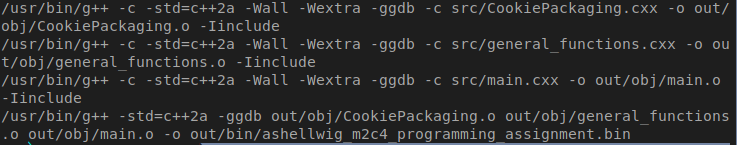
\includegraphics[%
        width={\textwidth}%
      ]{compile.png}
      \caption{Compiling Chapter 5`s Program}
      \label{img:compilation}
    \end{figure}
    \begin{figure}[H]
      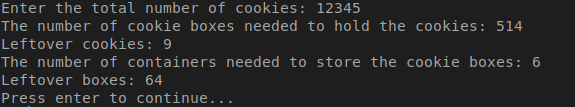
\includegraphics[%
        width={\textwidth}%
      ]{run.png}
      \caption{Running Chapter 5`s Program}
      \label{img:running}
    \end{figure}


  \newpage
  \section{Unit Tests}
    Tests were written with the
      \href{https://github.com/catchorg/catch}{Catch2 library}. The output is
      shown below.

    \begin{figure}[H]
      \caption{Test Output}
      \centering
      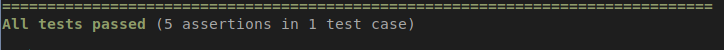
\includegraphics[width=\textwidth]{testout.png}
    \end{figure}
\end{document}\caption{Test Output}

